\documentclass{article}
\usepackage{fullpage}
\usepackage{graphicx}
\usepackage{hyperref}
\title{Information for SEA 2022}
\date{}
\begin{document}
\begin{center}
\begin{minipage}{5cm}
\vspace*{-2.4cm}
        
\includegraphics[width=6cm]{logo3}
        \end{minipage}
        \hspace*{1.5cm}
        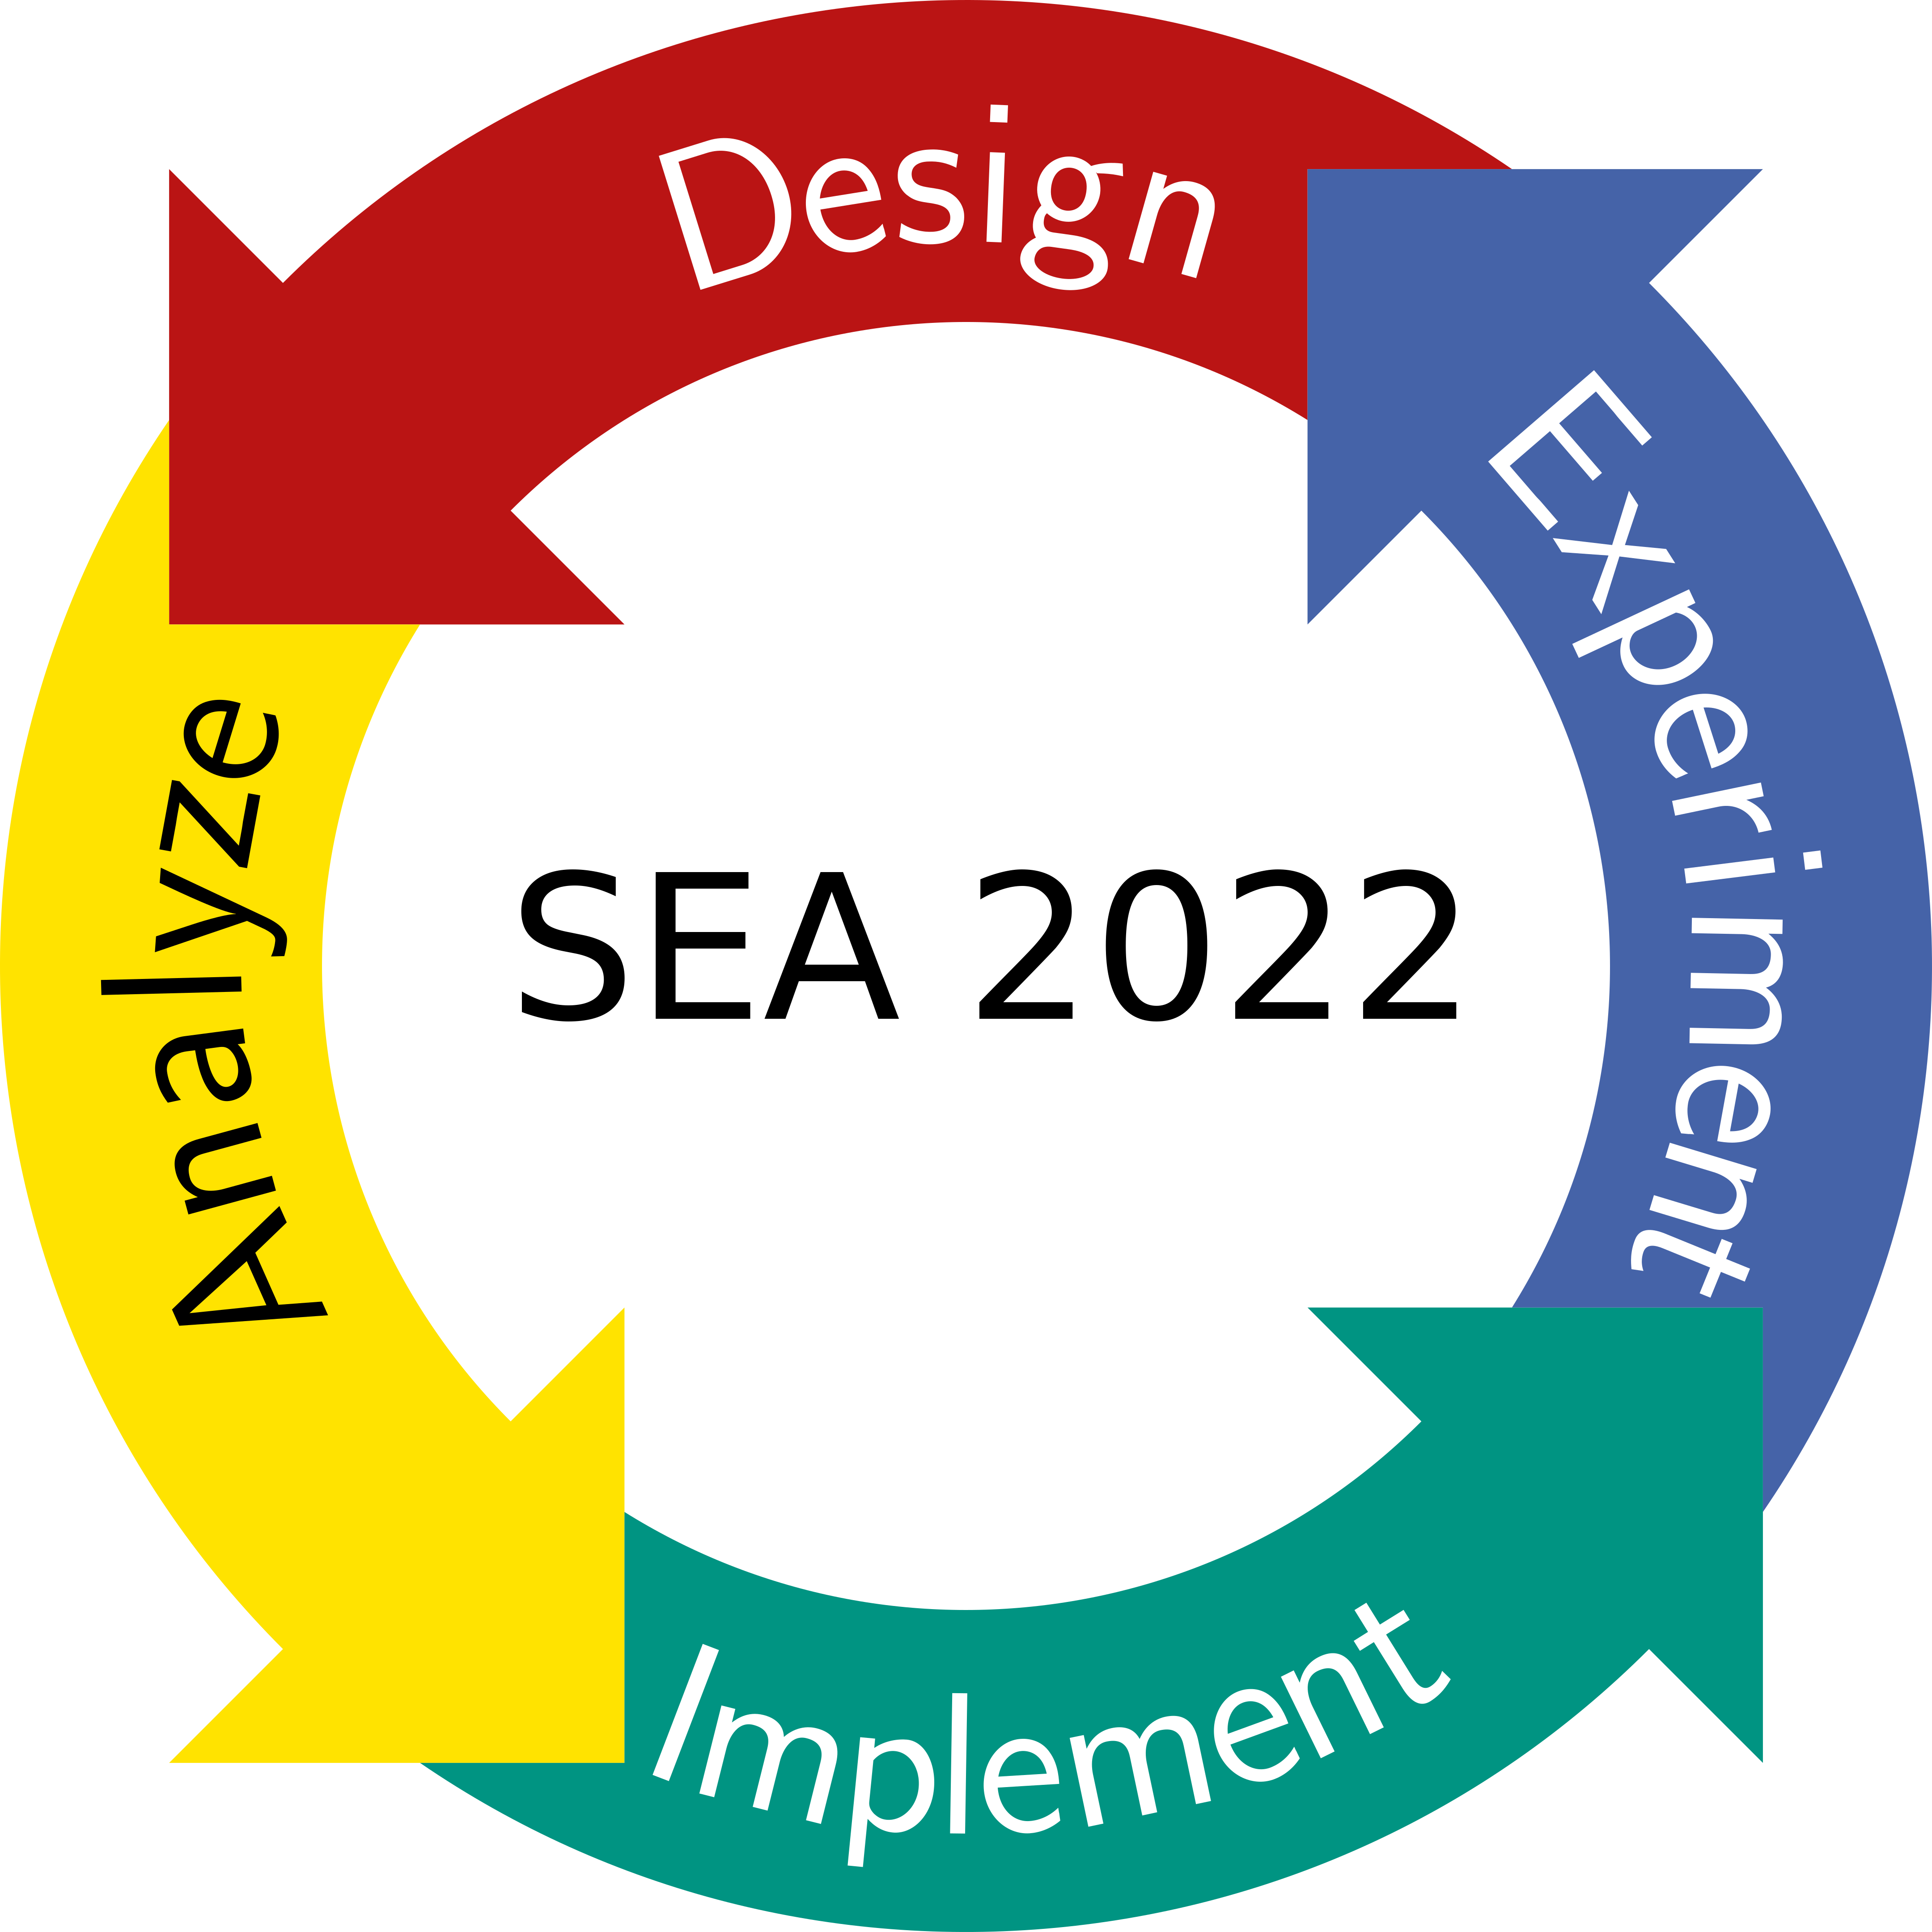
\includegraphics[width=2.85cm]{tasseentwurf_vec_sea}
        \hspace*{.5cm}
        
\includegraphics[width=5.3cm]{heidelberg-university.png}
\end{center}
%\maketitle
\section{Transport}
We recommend to buy the "9-Euro-Ticket" for July as this permits travel on buses, trams, and local trains within Germany in June inside Germany. 
\section{WLAN}
There is eduroam available. If you don't have access to eduroam, you may use Heidelberg4you which is a free Wifi provider thoughout the entire city.
\section{Corona}
One has to wear facemasks on German public transport. Similarly, the Heidelberg University requires facemasks inside buildings whenever there is another person within 1.5m to oneself. 

\section{Lunches}
Lunches will take place on level -1 of the Mathematikon building (the building of the conference). On each day, please bring the lunch voucher for the correct day that you received with your name tag.

\section{Monday / City Tour}
On Monday there will be a city tour (see schedule). The starting point of the city tour will be Löwenbrunnen near Universitätsplatz at 7:15pm (see \url{shorturl.at/eAKRX}). If you want to, we can walk there together, i.e. we will gather in front of the main entrance and we will leave the Mathematikon building at 6:30pm to walk over to the city tour starting spot. 
\begin{center}
        
\includegraphics[width=4cm]{qr-code_citytour.png}
\end{center}

\section{Tuesday / Hike}

On Tuesday we will do a hike via the famous Philosophenweg. The hike will end at the dinner location (see below). We will gather in front of the main entrance of the Mathematikon building and will leave the Mathematikon building at 5pm to start the hike. If you don't want to join the hike you can also directly come to the dinner location at 8pm.
\section{Tuesday / Dinner}
The dinner will take place on Tuesday starting from 8pm in the Heidelberg Castle (see \url{https://www.heidelberger-schloss-gastronomie.de/en/}; see also \url{shorturl.at/fkpMN}). Please bring your dinner voucher that you received with your name tag. 
\begin{center}
        
\includegraphics[width=4cm]{qr-code_schloss_location.png}
\end{center}

\section{Local Organisation Team}
The local organisation team consists out of Marcelo Fonseca Faraj, Ernestine Großmann, Catherine Proux-Wieland, Christian Schulz and Bora Uçar. If you have any question feel free to contact us at any time. You can also spot us by looking for a green mark on the name tag.

\section{Proceedings}
The conference proceedings can be found here \url{XXX}.
\vfill
\pagebreak
\section{WhatsApp}
We created a Whatsapp group for the event. Feel free to join via \url{shorturl.at/djGMU} or via scanning the following QR code:
\vspace*{1cm}

\begin{center}
        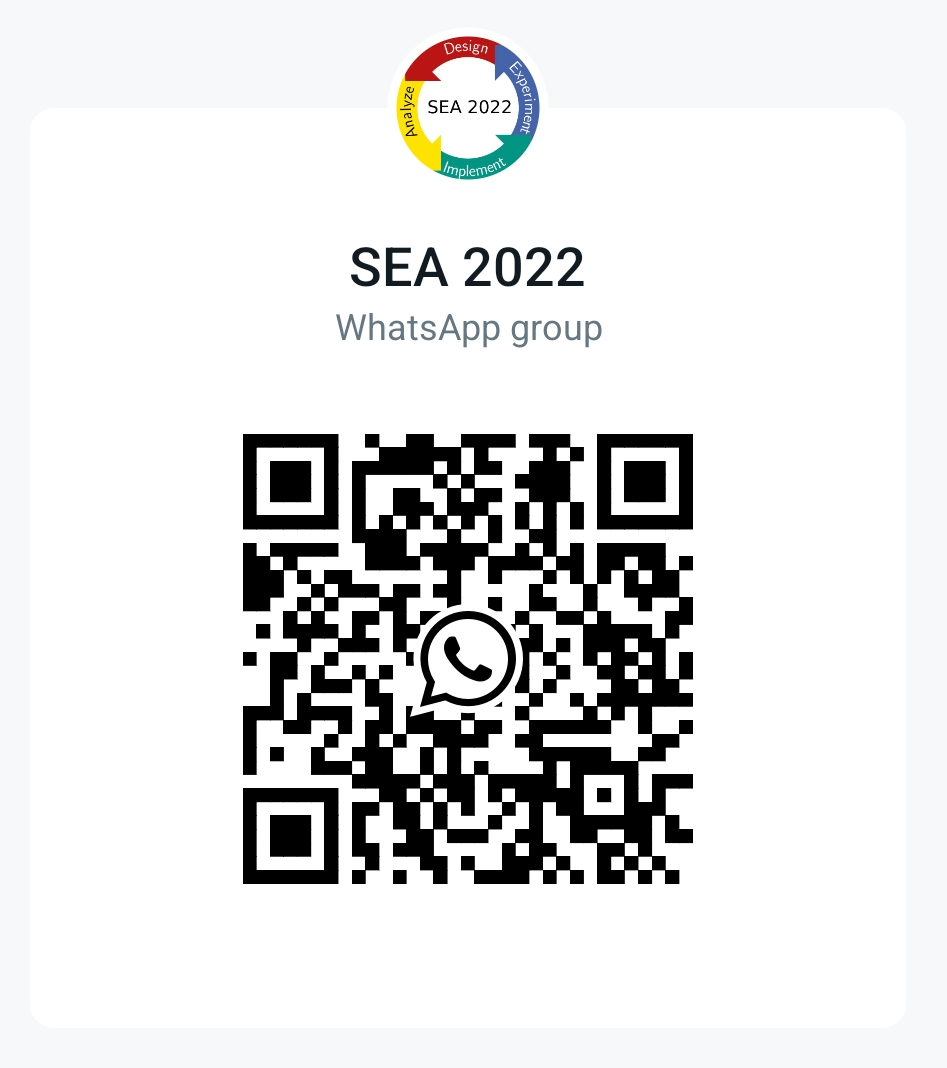
\includegraphics[width=9cm]{whatsapp.jpg}
\end{center}
\vfill
\pagebreak
\section{Program Monday}
\begin{center}
        \includegraphics[width=\textwidth]{programMonday.png}
\end{center}
\vfill
\pagebreak
\section{Program Tuesday}
\begin{center}
        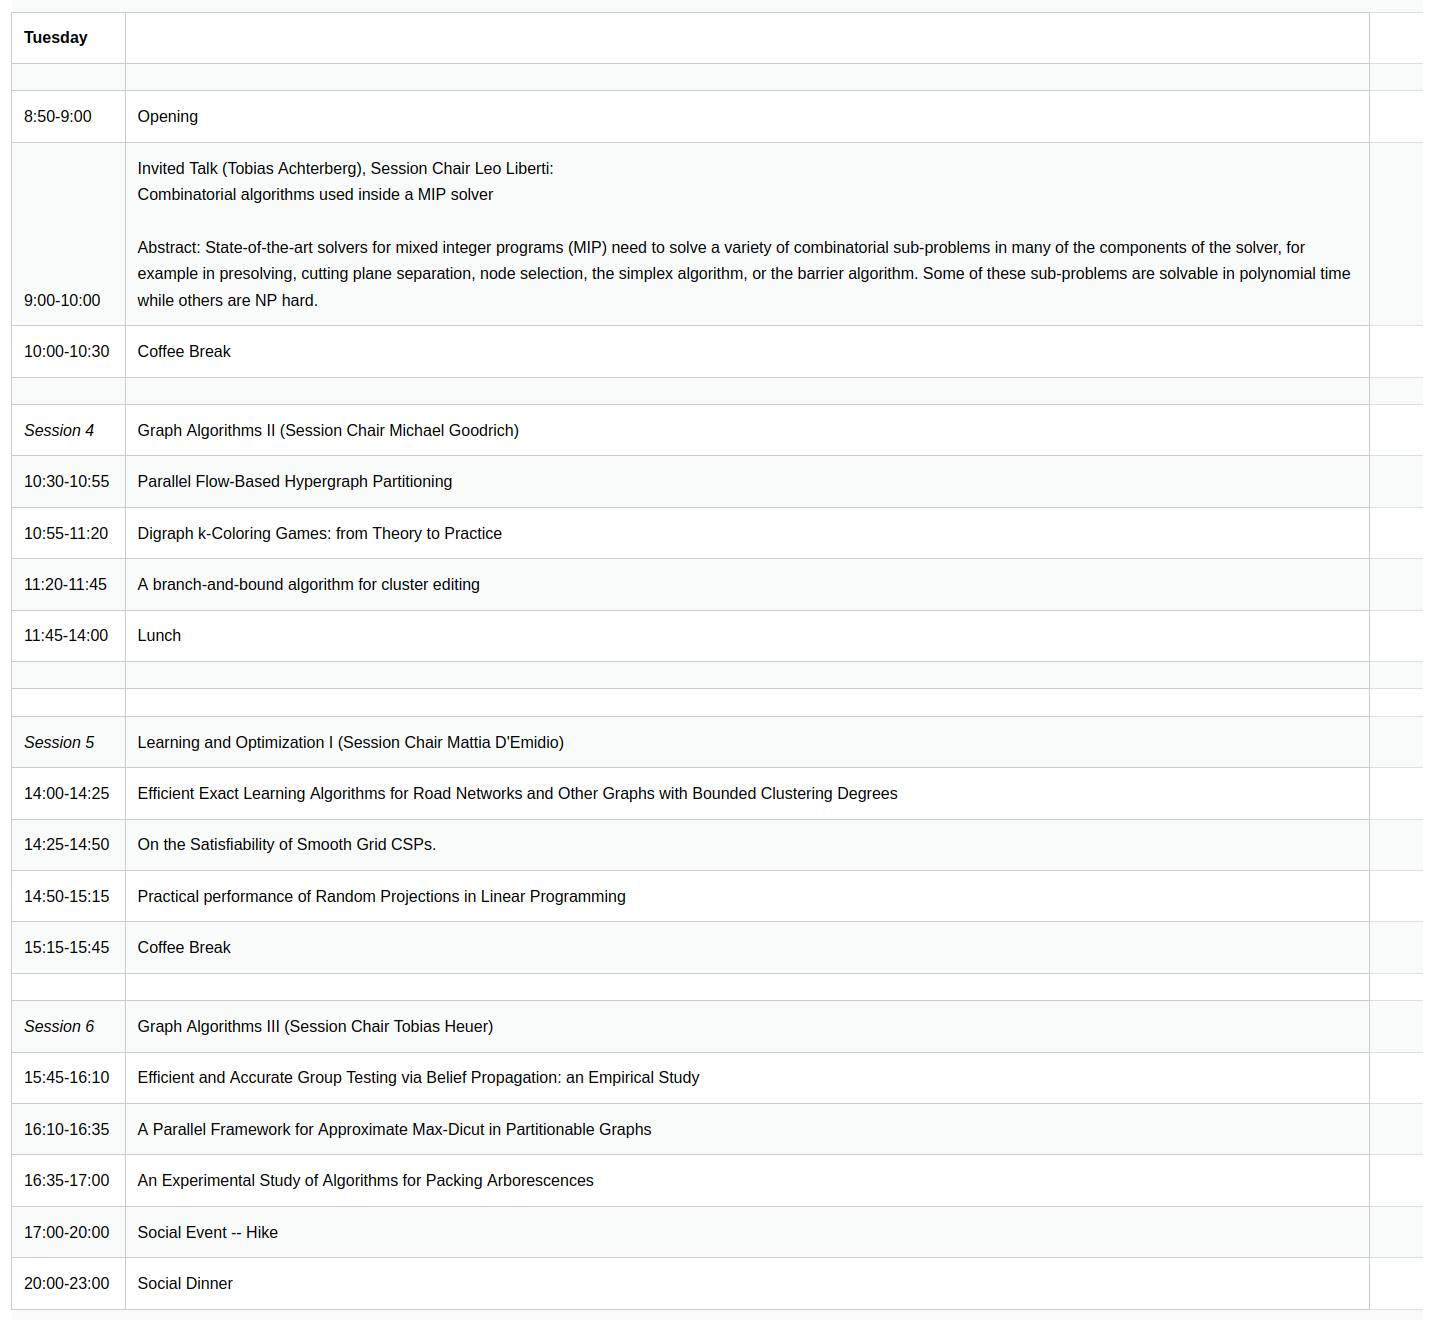
\includegraphics[width=\textwidth]{programTuesday.png}
\end{center}
\vfill
\pagebreak
\section{Program Wednesday}
\begin{center}
        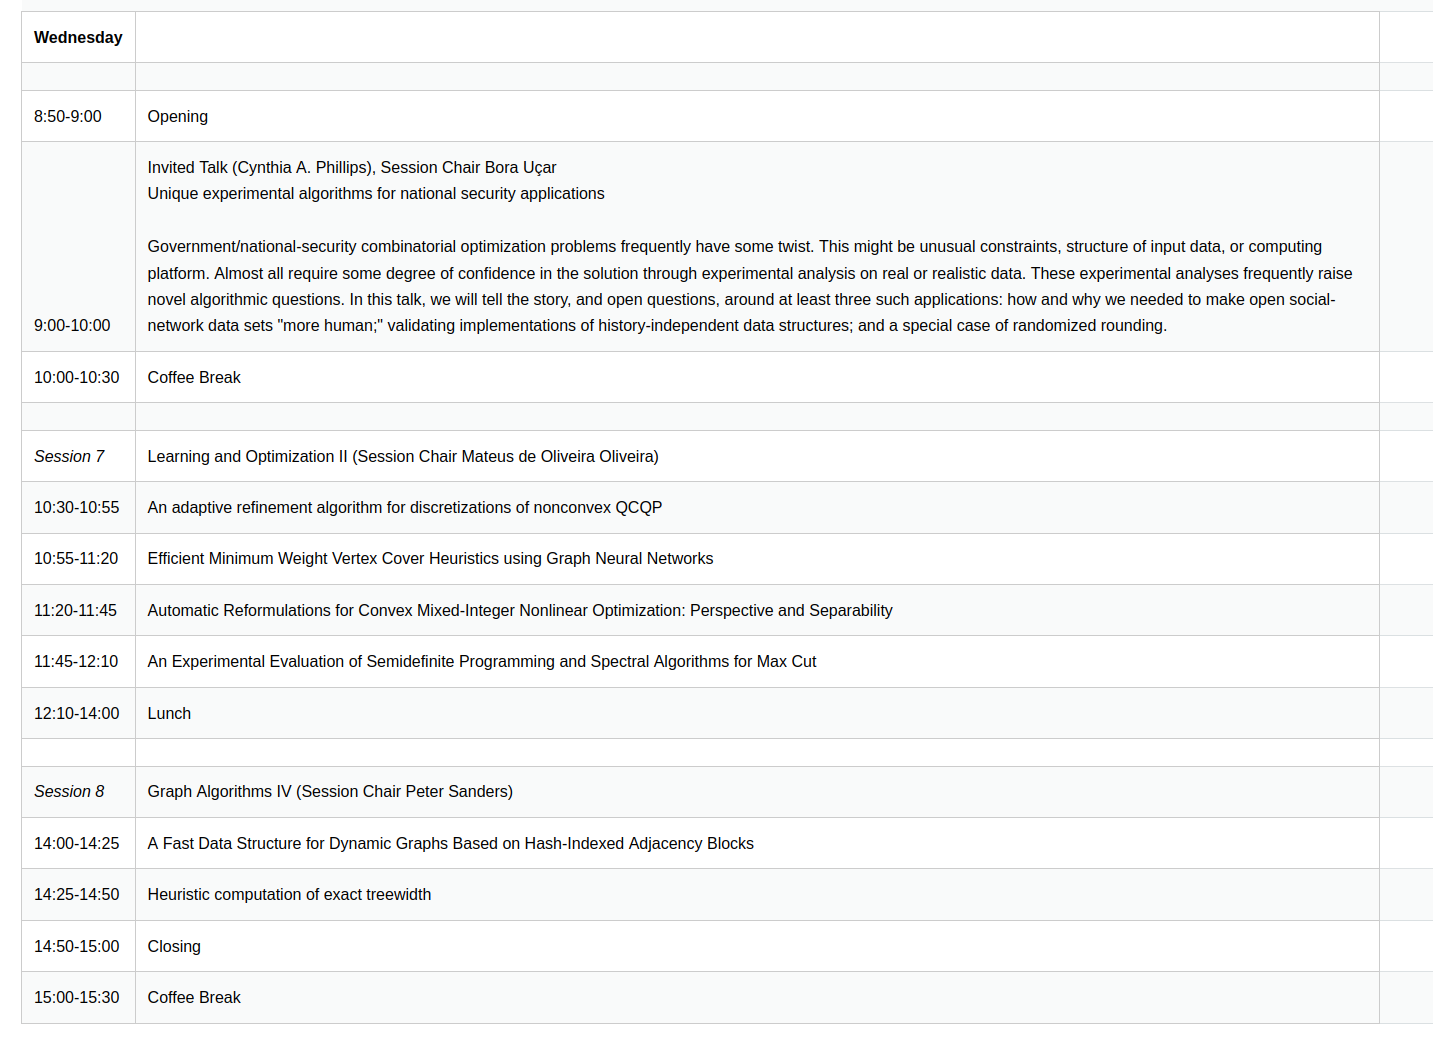
\includegraphics[width=\textwidth]{programWednesday.png}
\end{center}
\end{document}
